\subsection{Center-protected head and residual energy}\label{sec:protected-method}
The measured construction specializes the audit to public centers fixed before the query. Choose the first center $c_0$ as an anchor, and let $U\in\mathbb R^{d\times h}$ have orthonormal columns spanning all differences $c_j-c_0$, with $h\leq k-1$. Define
\begin{align}
w(x)&=x-c_0, & h(x)&=U^\top w(x),\\
r(x)&=(I-UU^\top)w(x), & e(x)&=\|r(x)\|^2.
\end{align}
The head directions are shared by every point; each point stores its own head coordinates. A sparse random tail $Ar(x)$ can additionally represent residual geometry, but the following identity determines which information is needed by the measured queries.

\begin{proposition}[Fixed-center sufficient statistics]\label{prop:head-energy}
For every point $x$ and every fixed center $c_j$,
\begin{equation}\label{eq:head-energy}
\|x-c_j\|^2=\|h(x)-h(c_j)\|^2+e(x).
\end{equation}
Consequently, the head alone determines the first-index nearest-center assignment, and the head together with one residual-energy value determines every fixed-center distance and their nearest-center sum.
\end{proposition}
\begin{proof}
Every $c_j-c_0$ lies in the column span of $U$. Thus
$x-c_j=U(h(x)-h(c_j))+r(x)$ is an orthogonal decomposition. Pythagoras gives Eq.~\eqref{eq:head-energy}. The same $e(x)$ is added for every candidate center, so the nearest-center comparisons and their ties depend only on the head.
\end{proof}

The ordinary protected representation stores $(h(x),Ar(x))$ and estimates cost using the tail's squared norm. The energy representation instead stores $(h(x),e(x),Ar(x))$ with total width 16 in the measured proof study. Its assignment and cost queries use only $(h(x),e(x))$. The matched no-JL control therefore stores exactly those $h+1$ values. The identity is exact in real arithmetic; the implemented query circuit proves an exact relation on rounded integers, which approximates the floating-point original-space costs.

For the completed proof study the owner commits quantized integer rows. The host uses $S=4096/\max(\max|X|,\max|\mathcal C|,10^{-12})$, rounds inputs and centers, and constructs $U$ from the quantized center differences. With $T=4096$ and $B_U=\operatorname{round}(TU^\top)$, the proved derivation is
\begin{align}
v&=B_U(x-c_0), & H&=Tv,\nonumber\\
R&=T^2(x-c_0)-B_U^\top v, & E&=\sum_\ell R_\ell^2,\label{eq:protected-integer}\\
J&=AR.\nonumber
\end{align}
The decoded head and residual are $H/T^2$ and $R/T^2$, with energy $E/T^4$. Costs are additionally divided by $S^2$. The no-JL control copies the same head and energy. Since $B_U/T$ is rounded, the proof is exact for this integer relation while its original-space distance identity is approximate. Input, coefficient, coordinate, energy, score and aggregate bounds prevent field wraparound. Precision effects are measured separately rather than assuming the real identity survives rounding exactly.

The tail is used only for separate pair geometry, with Euclidean features $(h(x),Ar(x))$; energy is not a Euclidean coordinate. Conditional on preserving every residual difference within relative squared-norm error $\epsilon$, the combined head/tail distance has absolute error at most $\epsilon\|r(x)-r(y)\|^2\leq\epsilon\|x-y\|^2$ by orthogonality. This statement does not supply a concentration bound for the tested one-sparse maps. At total budget 16, a rank-four head leaves eleven tail values after energy; rank nine leaves six. Shared model storage, authentication material and unequal statistic bit widths are excluded from these scalar counts.

\subsection{Implemented query relation and original-data binding}\label{sec:query-relation}
The implemented two-stage relation has an owner-supplied original catalog root $C_X$, a joint head/energy row root $C_H$, an optional separate tail root $C_T$, and a context hash binding these roots and the public model. The measurements use constant public centers. Stage 1 proves each original row's membership, its deterministic derivation in Eq.~\eqref{eq:protected-integer}, and membership of its resulting statistics under the output roots. The independent verifier requires every catalog index exactly once. Stage 2 takes public sorted distinct subset indices and a public claimed cost. Its private witness contains the authenticated rows, salts, paths and first-index assignments. The circuit opens head and energy together, checks ranges and deterministic center-score comparisons, and constrains
\begin{equation}
\widehat\Psi=\sum_{i\in I}\left(\|H_i-H(c_{a_i})\|^2+E_i\right).
\end{equation}
Here $I$ is the public subset and the integer sum is decoded by $T^4S^2$. Only the claimed sum, indices, commitments and model metadata are public; assignments remain witness values in the proof relation. The experiment saves assignment diagnostics privately for reference checking. Full opens original rows directly and needs no preprocessing proof.

Stage 1 also binds the optional tail; fixed-center Stage 2 leaves it unused. A separate pair-distance circuit opens both points' head/tail rows and proves their stored embedding distance, excluding energy. It does not prove original-space approximation quality. The trusted owner root, approved public model and verification-key hashes must come through an authentic channel. Center/PCA training, basis orthonormality/span approval and canonical challenge checks remain host/verifier obligations. In the main driver the tail is derived after the owner root from a locally held nonce allocated earlier; wider-tail follow-ups use a fresh nonce after the existing root. The 64-row catalog reuses the earlier approved matrix, so that run tests binding/performance rather than a fresh post-commit geometric draw. There is no deployed beacon, in-circuit XOF or general output-privacy guarantee.

Two exact task-specific controls are necessary for interpreting the speed result. With $w=x-c_0$ and $\delta_j=c_j-c_0$, exact affine stores $s_j=2\langle w,\delta_j\rangle-\|\delta_j\|^2$ for $j>0$ and $\beta=\|w\|^2$, with $s_0=0$. The winner maximizes $s_j$, and minimum cost is $\beta-\max_j s_j$. These $k$ values reproduce integer Full exactly. Cached exact answers instead prove and store just the nearest-center index and minimum cost during Stage 1, then authenticate/sum them for each subset. They support the fixed task more cheaply but do not supply arbitrary pair geometry. PCA is feasible in ZK: its baseline proves the approved projected calculation, while PCA training is outside the proof for this study.

\begin{figure*}[!htbp]
\centering
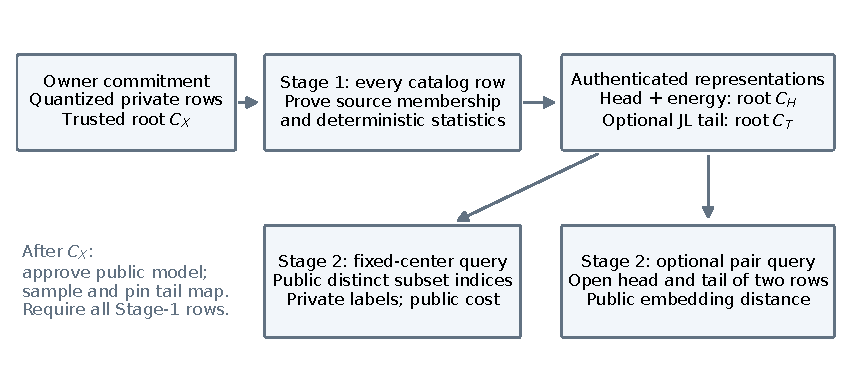
\includegraphics[width=0.94\textwidth]{paper_results/bound_revision/figures/protocol.pdf}
\caption{Measured construction and its trust boundary. Every original-to-statistic row is now proved in Stage 1; later subsets authenticate rows under fixed catalog roots. Tail geometry uses a separate query and root. Public-model approval and challenge policy remain external checks.}
\label{fig:measured-scope}
\end{figure*}
